\documentclass[a4paper,11pt]{article}

\usepackage{mlsubmit}
\usepackage{listings}

\begin{document}

\initmlsubmision{2} % assignment number
{Shashi Kant Gupta}   % your name
{160645}	% your roll number

\begin{mlsolution}
\noindent
According to the given problem:
\begin{equation}
  p(\vw) = C*exp(\frac{-\lambda}{2}\vw^{T}\vw)
\end{equation}
\begin{equation}
  p(\vy|\vX, \vw) = \prod_{n=1}^{N}\frac{1}{1 + exp(-y_{n}\vw^{T}\vx_{n})}
\end{equation}
Therefore, MAP estimate will be:
\begin{equation}
  \hat\vw_{MAP} = argmax_{\vw}log(p(\vy|\vX, \vw)) + log(p(\vw))
\end{equation}
\begin{equation}
  \Rightarrow \hat\vw_{MAP} = argmax_{\vw}\sum_{n=1}^{N}-log(1 + exp(-y_{n}\vw^{T}\vx_{n})) + \frac{-\lambda}{2}\vw^{T}\vw
\end{equation}
\begin{equation}
  \Rightarrow \hat\vw_{MAP} = argmin_{\vw}\sum_{n=1}^{N}log(1 + exp(-y_{n}\vw^{T}\vx_{n})) + \frac{\lambda}{2}\vw^{T}\vw
\end{equation}
Therefore, to minimise the negative log likelihood the partial derivatives w.r.t. to $\vw$ yields.
\begin{equation}
  \lambda\vw + \sum_{n=1}^{N}\frac{-y_{n}\vx_{n}exp(-y_{n}\vw^{T}\vx_{n})}{1 + exp(-y_{n}\vw^{T}\vx_{n})} = 0
\end{equation}
\begin{equation}
  \Rightarrow \hat\vw_{MAP} = \frac{1}{\lambda}\sum_{n=1}^{N}\frac{exp(-y_{n}\vw^{T}\vx_{n})}{1 + exp(-y_{n}\vw^{T}\vx_{n})}y_{n}\vx_{n}
\end{equation}
\begin{equation}
  \therefore \alpha_{n} = \frac{1}{\lambda}(\frac{exp(-y_{n}\vw^{T}\vx_{n})}{1 + exp(-y_{n}\vw^{T}\vx_{n})})
\end{equation}
From the expression of $\alpha_{n}$, we can see that it specifies an scaled version of non-class probabilities for $x{n}$. This make sense as we can see from the probability expression for the right-class as the $\alpha_{n}$ increases the probability for the right-class will increase, which means if probability of wrong-class is high it will give us a new estimate of $\vw$ such that probability of right class will increase.

\end{mlsolution}

\begin{mlsolution}

\noindent
As per the problem:
\begin{equation}
  p(y=1) = \pi
\end{equation}
\begin{equation}
  p(\vx|y=1) = \prod_{d=1}^{D}\mu_{d,1}^{xd}(1 - \mu_{d,1})^{1 - xd}
\end{equation}
\begin{equation}
  p(\vx|y=0) = \prod_{d=0}^{D}\mu_{d,0}^{xd}(1 - \mu_{d,0})^{1 - xd}
\end{equation}
\begin{equation}
  \therefore p(y=1|\vx) = \frac{\pi\prod_{d=1}^{D}\mu_{d,1}^{xd}(1 - \mu_{d,1})^{1 - xd}}{\pi\prod_{d=1}^{D}\mu_{d,1}^{xd}(1 - \mu_{d,1})^{1 - xd} +
  (1-\pi)\prod_{d=0}^{D}\mu_{d,0}^{xd}(1 - \mu_{d,0})^{1 - xd}}
\end{equation}
\begin{equation}
  = \frac{1}{1 + \frac{1-\pi}{\pi}\prod_{d=1}^{D}{[\frac{\mu_{d,0}}{\mu_{d,1}}]}^{\vx_{d}}
  {[\frac{1 - \mu_{d,0}}{1-\mu_{d,1}}]}^{1-\vx_{d}} }
\end{equation}
\begin{equation}
  = \frac{1}{1+f(\vx)}
\end{equation}
where $f(\vx) = \frac{1-\pi}{\pi}\prod_{d=1}^{D}{[\frac{\mu_{d,0}}{\mu_{d,1}}]}^{\vx_{d}}
{[\frac{1 - \mu_{d,0}}{1-\mu_{d,1}}]}^{1-\vx_{d}}$
\\It can be easily shown that:
\begin{equation}
  p(y=0|\vx) = \frac{1}{1+f(\vx)^{-1}}
\end{equation}
Therefore, this makes a discriminative model with its distribution as $Bernoulli[g(f(\vx))]$
\\where $g(f(\vx)) = \frac{1}{1+f(\vx)}$ and $f(\vx) = \frac{1-\pi}{\pi}\prod_{d=1}^{D}{[\frac{\mu_{d,0}}{\mu_{d,1}}]}^{\vx_{d}}
{[\frac{1 - \mu_{d,0}}{1-\mu_{d,1}}]}^{1-\vx_{d}}$
\\
\\
\\For the decision boundary we can equate $p(y=1|\vx) = p(y=0|\vx)$. Which gives:
\begin{equation}
  \pi\prod_{d=1}^{D}\mu_{d,1}^{xd}(1 - \mu_{d,1})^{1 - xd} =
  (1-\pi)\prod_{d=0}^{D}\mu_{d,0}^{xd}(1 - \mu_{d,0})^{1 - xd}
\end{equation}
Or equivalently we can write, $f(\vx) = 1$ as the decision boundary! Therefore, here we get an exponential decision boundary!

\end{mlsolution}

\begin{mlsolution}

\noindent Let us first solve the Lagrangian for the given condition. We get:
\begin{equation}
  \hat\vw = argmax_{\lambda}[argmin_{w}[(\vy - \vX\vw)^{T}(\vy - \vX\vw) + \lambda(\vw^{T}\vw - C)]]
\end{equation}
Solving the above dual problem for argmin case we get:
\begin{equation}
  -2\vX^{T}(\vy - \vX\vw) + 2\lambda\vw = 0
\end{equation}
\begin{equation}
  \Rightarrow \vw = (\vX^{T}\vX + \lambda\vI)^{-1}\vX^{T}\vy
\end{equation}
If we recall the solution for the $l_{2}$ regularized least square linear regression model. There also we got the similar solution for with $\lambda$ being the hyperparameter for the regularization term! Therefore solving the above dual problem completly and finding the value for $\lambda$ will gives us the equivalent $l_{2}$ regularized solution! If we use the same $\lambda$ as the hyperparameter.


\end{mlsolution}

\begin{mlsolution}

\noindent As per the problem $p(\vy|\vx, \vW)$ can be written as:
\begin{equation}
  p(\vy|\vx, \vW) = \prod_{n=1}^{N}\prod_{k=1}^{K}{[\frac{exp(\vw^{T}_{k}\vx_{n})}{\sum_{l=1}^{K}
  exp(\vw^{T}_{l}\vx_{n})}]}^{1\{y_{n}=k\}}
\end{equation}
where, $1\{y_{n}=k\}$ is equal to $1$ when $y_{n}=k$ and $0$ when $y_{n}\neq k$. Therefore, taking the loglikelihood give us:
\begin{equation}
  LL(\vw) = \sum_{n=1}^{N}\sum_{k=1}^{K}1\{y_{n}=k\}log(\frac{exp(\vw^{T}_{k}\vx_{n})}{\sum_{l=1}^{K}exp(\vw^{T}_{l}\vx_{n})})
\end{equation}
\begin{equation}
  = \sum_{n=1}^{N}1\{y_{n}=k\}log(\frac{exp(\vw^{T}_{k}\vx_{n})}{\sum_{l=1}^{K}exp(\vw^{T}_{l}\vx_{n})}) +
  \sum_{n=1}^{N}1\{y_{n}\neq k\}log(1 - \frac{exp(\vw^{T}_{k}\vx_{n})}{\sum_{l=1}^{K}exp(\vw^{T}_{l}\vx_{n})})
\end{equation}
\begin{equation}
  \Rightarrow \frac{LL(\vw)}{\partial \vw} =
  \sum_{n=1}^{N}1\{y_{n}=k\}\vx_{n}(1- \frac{exp(\vw^{T}_{k}\vx_{n})}{\sum_{l=1}^{K}exp(\vw^{T}_{l}\vx_{n})}) +
  \sum_{n=1}^{N}1\{y_{n}\neq k\}(-\vx_{n}\frac{exp(\vw^{T}_{k}\vx_{n})}{\sum_{l=1}^{K}exp(\vw^{T}_{l}\vx_{n})})
\end{equation}
\begin{equation}
  = \sum_{n=1}^{N}\vx_{n}(1\{y_{n}=k\} -\frac{exp(\vw^{T}_{k}\vx_{n})}{\sum_{l=1}^{K}exp(\vw^{T}_{l}\vx_{n})})
\end{equation}
Therefore GD update rule will be:
\begin{equation}
  \vw_{k}^{t+1} = \vw_{k}^{t} + \frac{1}{N}\sum_{n=1}^{N}\vx_{n}(1\{y_{n}=k\} -\frac{exp(\vw^{t,T}_{k}\vx_{n})}{\sum_{l=1}^{K}exp(\vw^{t,T}_{l}\vx_{n})})
\end{equation}
SGD update rule will be:
\begin{equation}
  \vw_{k}^{t+1} = \vw_{k}^{t} + \vx_{n}(1\{y_{n}=k\} -\frac{exp(\vw^{t,T}_{k}\vx_{n})}{\sum_{l=1}^{K}exp(\vw^{t,T}_{l}\vx_{n})})
\end{equation}
\begin{equation}
   = \vw_{k}^{t} + \vx_{n}(1\{y_{n}=k\} - \mu_{nk})
\end{equation}
\\
\\SGD Algorithm:
\begin{lstlisting}
for k in range(K):
  while not converges:
    i = rand(1,N);
    p = exp(dot(w[k].T, x[i])/sum(exp(dot(W,x[i])));
    if y[i] == k:
      w[k] = w[k] + x[i]*(1 - p)
    else:
      w[k] = w[k] - x[i]*(p)

\end{lstlisting}
\\
\\
\\For the hard class case. $\mu_{nk}$ of sgd will change to our new $\mu_{nk}$. Which can be written as: $\prod_{j=1}^{K} 1\{\vw_{k}^{T}\vx > \vw_{j}^{T}\vx\}$
Therefore, our new SGD update rule will be:
\begin{equation}
   \vw_{k}^{t+1} = \vw_{k}^{t} + \vx_{n}(1\{y_{n}=k\} - \prod_{j=1}^{K} 1\{\vw_{k}^{T}\vx > \vw_{j}^{T}\vx\})
\end{equation}
\\
\\SGD Algorithm:
\begin{lstlisting}
while not converges:
  i = rand(1,N);
  if y[i] == argmax(dot(W, x[i])):
    w[y[i]] = w[y[i]] + x[i]
  else:
    w[y[i]] = w[y[i]] - x[i]
\end{lstlisting}

\end{mlsolution}


\begin{mlsolution}

\noindent We say two sets $\{\vx_{n}\}$ and $\{\vy_{n}\}$ are linear separable if we can find $\vw$ and $\vb$ such that: \\$\vw^{T}\vx_{n} + \vb > 0$ and $\vw^{T}\vy_{n} + \vb < 0$ for every $\vy_{n}$ and $\vx_{n}$. Now lets prove the given statement!
\\
\\Case 1: $Convex Hull Intersects \Rightarrow Not Seperable$
\\If the two convex hull intersects then we can find a common point $\vz$ such that:
\begin{equation}
  \vw^{T}\vz + \vb = \vw^{T}\sum_{n=1}\alpha_{n}\vx_{n} + \vb > 0
\end{equation}
Also:
\begin{equation}
  \vw^{T}\vz + \vb = \vw^{T}\sum_{n=1}\alpha_{n}\vy_{n} + \vb < 0
\end{equation}
But they both contradicts each other, therefore this means $\vx_{n}$ and ${\vy_{n}}$ are not seperable!
\\
\\Case 2: $Seperable \Rightarrow Convex Hull Not Intersects$
\\Since they are seperable if a point $\vz$ lies inside the convex hull of $\vx_{n}$ then it will satisfy:
\begin{equation}
  \vw^{T}\vz + \vb = \vw^{T}\sum_{n=1}\alpha_{n}\vx_{n} + \vb > 0
\end{equation}
And if a point $\vz^{'}$ lies inside the convex hull of $\vy_{n}$ then it will satisfy:
\begin{equation}
  \vw^{T}\vz^{'} + \vb = \vw^{T}\sum_{n=1}\alpha_{n}\vy_{n} + \vb < 0
\end{equation}
Therefore, $\vz^{'}$ will never be equal to $\vz$. Which means the convex hull will not intersects!

\end{mlsolution}

\begin{mlsolution}

\noindent Writing the lagrangian objective function for this case:
\begin{equation}
  \vL(\vw, \vb, \alpha_{n}) = \frac{||\vw||^{2}}{2} + \sum_{n=1}^{N}\alpha_{n}(m - y_{n}(\vw^{T}\vx_{n}+\vb))
\end{equation}
Now, substituting $\vw = m\vw_{s}$ and $\vb = m\vb_{s}$ in the above objective our new objective can be written as:
\begin{equation}
  \vL(\vw, \vb, \alpha_{n}) = \frac{||\vw_{s}||^{2}}{2} + \sum_{n=1}^{N}\alpha_{n}(m - y_{n}(m\vw^{T}_{s}\vx_{n}+m\vb_{s}))
\end{equation}
\begin{equation}
  = \frac{||\vw_{s}||^{2}}{2} + \sum_{n=1}^{N}m\alpha_{n}(1 - y_{n}(\vw^{T}_{s}\vx_{n}+\vb_{s}))
\end{equation}
\begin{equation}
  = \frac{||\vw_{s}||^{2}}{2} + \sum_{n=1}^{N}\alpha_{s,n}(1 - y_{n}(\vw^{T}_{s}\vx_{n}+\vb_{s}))
\end{equation}
where $\alpha_{s,n}=m\alpha_{n}$.
\\This come out to be the same objective as that for the SVM case. Therefore, the parameter learned in this newer case will be $\vw = m\vw_{s}$ $\vb = m\vb_{s}$. Therefore the newer seperating hyperplane will be:
\begin{equation}
  \vw^{T}\vx + \vb = 0
\end{equation}
\begin{equation}
  \Rightarrow m(\vw^{T}_{s}\vx + \vb_{s}) = 0
\end{equation}
which is the same hyperplane as that for the SVM case!

\end{mlsolution}

\begin{mlsolution}
  \noindent For the second part when binclassv2.txt was used which contains some outliers points for the red points.
  \\In generative case, the decision boundary comes more close to the blue clusters, possible reason could be that since sigma variance for red will increase due to the outliers so the boundary will come closer to the blue one.\\
  But for SVM case there was a little shift toward red clusters, possibly due to increase in the no of red crossovers the new decision had tried to shift a little to decrease other crossovers! which we can see from the image that there is more no of points on the decision boundary for part2\\
  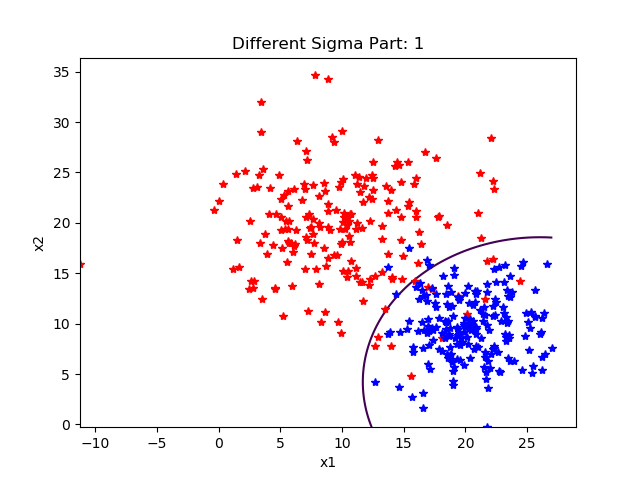
\includegraphics{Figure_1}
  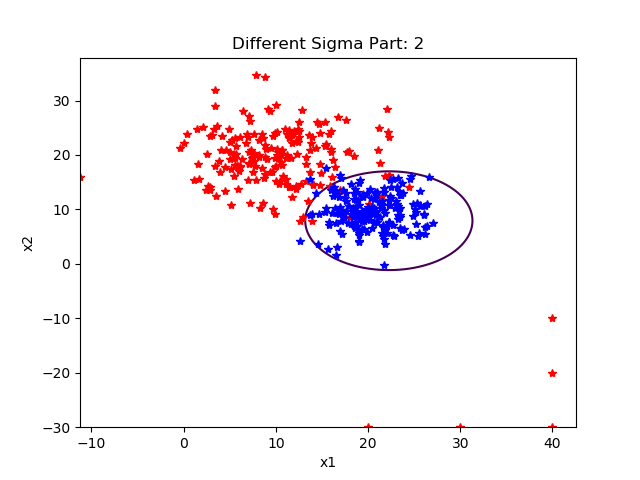
\includegraphics{Figure_12}
  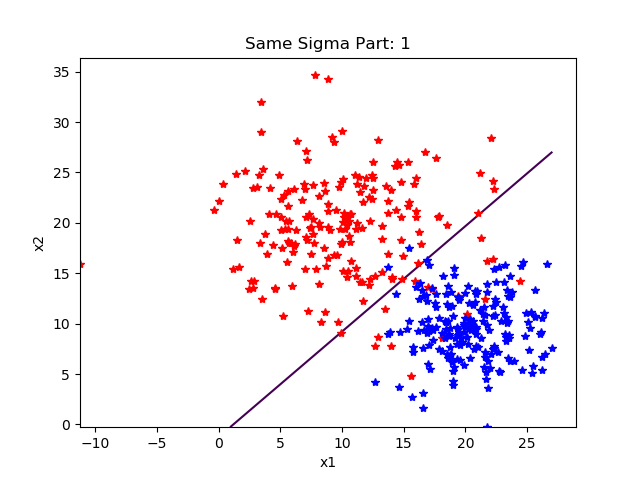
\includegraphics{Figure_2}
  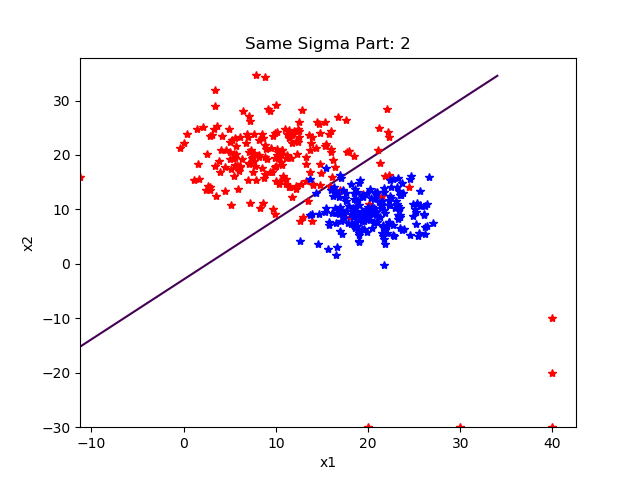
\includegraphics{Figure_22}
  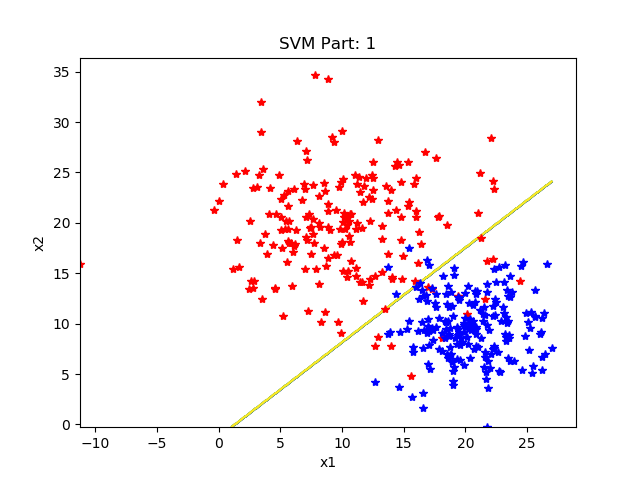
\includegraphics{Figure_svm1}
  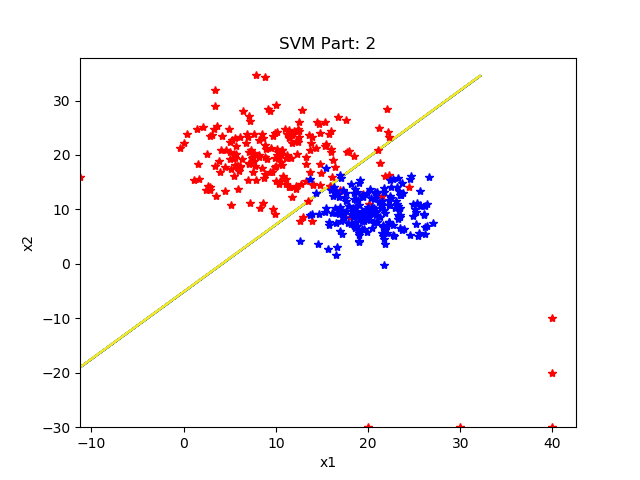
\includegraphics{svm2}
\end{mlsolution}


\end{document}
